\RequirePackage{luatex85}
\documentclass[tikz,border=0]{standalone}
\usepackage[no-math]{fontspec}
\setmainfont[Ligatures=TeX]{PragmataPro-Bold}
\usetikzlibrary{bayesnet,positioning,backgrounds,fit}
\definecolor{bgColor}{RGB}{38,50,56}
\definecolor{textColor}{RGB}{195,206,227}
\definecolor{nodeColor}{RGB}{195,206,227}
\definecolor{edgeColor}{RGB}{195,206,227}
\begin{document}
  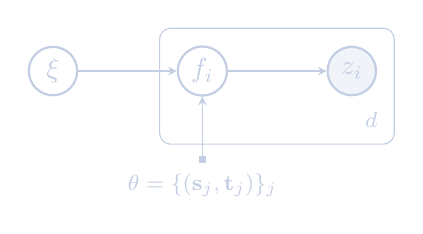
\begin{tikzpicture}[textColor]
  	\tikzstyle{latent} = [circle,draw=nodeColor,thick,inner sep=2pt,minimum size=1.75em,node distance=1]
  	\tikzstyle{obs} = [latent,draw=nodeColor,fill=textColor,fill opacity=.25,text opacity=1]
  	\tikzstyle{factor} = [rectangle,fill=nodeColor,minimum size=.25em,inner sep=0pt,node distance=0.4]
  	\tikzstyle{plate} = [draw,rectangle,rounded corners,inner sep=6pt,fit=#1]
  	\tikzset{>={stealth}}

	  \node [obs] (zi) {$z_i$};
	  \node [latent, left=1.25cm of zi] (fi) {$f_i$};
	  \node [latent, left=1.25cm of fi] (xi) {$\mathbf{\xi}$};

	  \factor [below=.75cm of fi] {theta} {below:$\mathbf{\theta} = \{({\mathbf{s}_j}, {\mathbf{t}_j})\}_j$} {} {};
	  %\node [const, above=1cm of fi] (theta) {$\mathbf{\theta} = \{({\mathbf{s}_j}, {\mathbf{t}_j})\}_j$};

		\edge	{fi} {zi};
		\edge {xi,theta} {fi};

	  \plate {fizi} {(fi)(zi)} {$d$} ;

    % \begin{scope}[on background layer]
    %   \node [fill=bgColor,fit=(fizi) (theta) (theta-caption) (xi)] {};
    % \end{scope}
  \end{tikzpicture}
\end{document}